% ------------------------------------------------------------
% Template ATCC (Artigo de Conclusão de Curso) - Normas ABNT
% Baseado no arquivo "TCC_3 - Modelo ATCC.docx"
% Compilar com: pdflatex -> bibtex -> pdflatex -> pdflatex
% (No Overleaf: Menu > Compiler = pdfLaTeX; o bibtex roda sozinho)
% ------------------------------------------------------------
\documentclass[
	article,		% artigo cientifico (nao TCC completo)
	12pt,			% fonte 12pt, como no modelo
	oneside,
	a4paper,
	brazil
]{abntex2}

% ------------------------------------------------------------
\usepackage[
	top=3cm, left=3cm, right=2cm, bottom=2cm,
	headheight=2.8cm, headsep=0.6cm, footskip=1.25cm
]{geometry}

% ------------------------------------------------------------
% Pacotes
% ------------------------------------------------------------
\usepackage[utf8]{inputenc}
\usepackage[T1]{fontenc}
\usepackage{lmodern}
\usepackage{times}
\usepackage{indentfirst}
\usepackage{graphicx}
\usepackage{microtype}
\usepackage{booktabs}
\usepackage{multirow}
\usepackage{caption}
\usepackage{color}
\usepackage{fancyhdr}
\usepackage{amsmath}

% ------------------------------------------------------------
\usepackage[
	alf,
	abnt-emphasize=bf,
	abnt-etal-list=0,
	abnt-etal-cite=3,
	abnt-repeated-author-omit=no
]{abntex2cite}

% ------------------------------------------------------------
\pagestyle{fancy}
\fancyhf{}
\renewcommand{\headrulewidth}{0.4pt}
\renewcommand{\footrulewidth}{0pt}

\newcommand{\logocabecalho}{%
	\IfFileExists{imagens/logo-unicuritiba.png}%
		{
\includegraphics[height=2.2cm]{imagens/logo-unicuritiba.png}}%
		{\fbox{\parbox[c][2.2cm][c]{5cm}{\centering logo da Unicuritiba aqui}}}%
}
\fancyhead[C]{\logocabecalho}

\fancyfoot[L]{}
\fancyfoot[C]{}
\fancyfoot[R]{\thepage}

\fancypagestyle{primeirapagina}{%
	\fancyhf{}
	\fancyhead[C]{\logocabecalho}
	\renewcommand{\headrulewidth}{0.4pt}
	\renewcommand{\footrulewidth}{0pt}
}

% ------------------------------------------------------------
% Dados do artigo
% ------------------------------------------------------------
% TODO: confirmar nome exato do curso/instituicao e e-mail para a
% versao final -- preenchidos aqui com o melhor dado disponivel no
% repositorio (git config do autor).
\titulo{Extração de equações interpretáveis de redes neurais em grafo para identificação de um sistema MIMO de abastecimento de água}
\autor{Rodrigo Watanabe Pisaia\textsuperscript{1}}
\local{Curitiba, Brasil}
\data{\today}
\orientador{Prof. Dr. Aron Luiz Oliveira dos Santos}
\instituicao{Centro Universitário Curitiba (Unicuritiba) -- Engenharia} % TODO: confirmar nome exato do curso

% ------------------------------------------------------------
\begin{document}

\thispagestyle{primeirapagina}

\begin{center}
	{\large\bfseries \imprimirtitulo}\\[12pt]

	\imprimirautor\\
	\small rodrigo.watanabe0107@gmail.com\\[10pt] % TODO: confirmar e-mail institucional

	\normalsize Professor orientador: \imprimirorientador\\[10pt]

	\imprimirinstituicao
\end{center}

\vspace{12pt}

% ------------------------------------------------------------
% RESUMO
% ------------------------------------------------------------
\begin{center}
	\bfseries Resumo
\end{center}

\begin{SingleSpace}
\noindent Modelos caixa-preta de identificação de sistemas, como redes
neurais, costumam superar modelos lineares clássicos em acurácia, mas não
produzem uma equação que possa ser inspecionada ou usada em projeto de
controle. Este trabalho propõe e avalia um método de extração de equações
interpretáveis a partir de uma rede neural em grafo (\textit{Graph Neural
Network}, GNN) treinada para identificar um sistema MIMO de abastecimento
de água do reservatório São José (Sanepar), com quatro entradas (frequência
de três bombas e vazão de entrada) e três saídas (vazão de distribuição,
nível e pressão). O método baseia-se em uma \textit{Message Passing Neural
Network} cuja função de mensagem recebe apenas variáveis físicas nomeadas
(janelas de defasagem de cada série), em vez de um vetor latente sem nome,
e é regularizada por penalidade L1 para que a mensagem aprendida vire uma
transformação linear da interação verdadeira entre as variáveis.
Regressão simbólica é então aplicada separadamente sobre a função de
mensagem e sobre a função de atualização do modelo treinado, produzindo
expressões fechadas candidatas a lei física. Em paralelo, a norma da
mensagem por aresta fornece uma matriz de topologia de acoplamento, validada
contra causalidade de Granger e identificação ARX clássica. Resultados
preliminares de acurácia mostram que as arquiteturas em grafo superam o
ARMAX de referência (120 parâmetros) em previsão de 12 passos nas três
saídas, com a variante regularizada (\textit{message\_dim}=8) obtendo o
melhor desempenho em vazão e pressão entre as redes testadas. A extração
simbólica da equação permanece em andamento; o artigo documenta o método,
a implementação (disponível como pacote Python) e os resultados de
acurácia já obtidos como base para a etapa de destilação.

\vspace{6pt}
\noindent\textbf{Palavras-chave}: Identificação de sistemas. Redes neurais
em grafo. Regressão simbólica. Sistemas MIMO. Interpretabilidade.
\end{SingleSpace}

\vspace{12pt}

% ------------------------------------------------------------
% 1 INTRODUCAO
% ------------------------------------------------------------
\section{Introdução}

Sistemas de abastecimento de água municipal, como estações de bombeamento
e reservatórios, são sistemas dinâmicos de múltiplas entradas e múltiplas
saídas (MIMO) cuja operação eficiente depende de modelos matemáticos
confiáveis. \citeonline{ferrari2025} identificaram um sistema desse tipo --
o reservatório São José, operado pela Sanepar em Curitiba -- usando um
modelo ARMAX de ordem 3 com aproximadamente 120 parâmetros, ajustado por
metaheurísticas multiobjetivo (NSGA-II, MOGWO, MOCS). O modelo obtido é
preciso (R² entre 0,84 e 0,96 na validação), mas é, nas palavras dos
próprios autores, uma estrutura polinomial genérica sem relação direta com
a física do processo -- não há equação que relacione as saídas ao balanço
de massa do reservatório ou à curva das bombas.

Esse é precisamente o tipo de lacuna que métodos recentes de destilação
simbólica de redes neurais se propõem a fechar.
\citeonline{cranmer2020} mostraram que, ao treinar uma rede neural com uma
estrutura interna separável -- uma \textit{Graph Network}
\cite{battaglia2018} -- e regularizar o componente de mensagem entre nós,
é possível depois substituir esse componente por uma expressão simbólica
obtida via regressão simbólica, recuperando leis físicas conhecidas (leis
de força, por exemplo) a partir apenas dos dados, e até descobrindo uma
fórmula nova para a concentração de matéria escura em simulações
cosmológicas. O ganho central do método é fatorar o problema: em vez de
buscar simbolicamente sobre a rede inteira, busca-se sobre funções internas
pequenas, cada uma com poucas entradas.

Este trabalho aplica essa ideia ao sistema do reservatório São José. A
pergunta de pesquisa não é apenas \emph{prever} as três saídas do sistema,
mas \emph{extrair uma equação interpretável} que explique o acoplamento
entre as variáveis -- e, secundariamente, a topologia desse acoplamento
(quais entradas afetam quais saídas). A hipótese de trabalho é que um
modelo de identificação em grafo, mais simples que uma GNN "profunda" e
pensado desde o início para a extração, consegue (i) igualar ou superar a
acurácia do ARMAX de referência com uma ordem de grandeza menos parâmetros
e (ii) produzir uma expressão simbólica que recupere, pelo menos
qualitativamente, o balanço de massa conhecido do reservatório
($A\, dy_2/dt = u_4 - y_1$).

O restante do artigo está organizado da seguinte forma: a Seção 2 revisa
os fundamentos de redes de mensagens, destilação simbólica e explicação de
GNNs; a Seção 3 descreve os dados, a arquitetura proposta e o método de
extração; a Seção 4 apresenta os resultados de acurácia obtidos até o
momento e discute o estado da extração simbólica; a Seção 5 conclui.

% ------------------------------------------------------------
% 2 REFERENCIAL TEORICO
% ------------------------------------------------------------
\section{Referencial teórico}

\subsection{Identificação de sistemas MIMO e o caso do reservatório São José}

Identificação de sistemas é o processo de construir um modelo matemático de
um sistema dinâmico a partir de dados de entrada e saída observados
\cite{ljung1999}. Para sistemas multivariáveis, ferramentas clássicas como
o \textit{Relative Gain Array} (RGA) \cite{bristol1966, skogestad2005} e a
causalidade de Granger \cite{granger1969} permitem quantificar o
acoplamento entre pares entrada-saída sem assumir uma estrutura de modelo
específica, e servem de referência independente para validar a topologia
que um modelo mais complexo aprender.

O sistema-alvo deste trabalho é o reservatório São José (Sanepar,
Curitiba/PR), com quatro entradas -- frequência das bombas 1, 2 e 3 (Hz) e
vazão de entrada (l/s) -- e três saídas -- vazão de distribuição (l/s),
nível do reservatório (m) e pressão (mca), amostradas a cada hora.
\citeonline{ferrari2025} ajustaram a esse sistema um modelo ARMAX MIMO de
ordem 3, com 120 parâmetros estimados por seis metaheurísticas distintas,
usando 1.100 das 2.216 amostras disponíveis. O nível do reservatório foi a
saída mais difícil de ajustar: estratégias mono-objetivo produziram R²
negativo (até $-15{,}9$), o que os autores atribuem à diferença de ordem de
grandeza entre as saídas na agregação do erro. A física conhecida do
sistema é simples -- um balanço de massa de primeira ordem no nível,
$A\, dy_2/dt = u_4 - y_1$, e relações quase algébricas de perda de carga
para vazão e pressão -- mas essa estrutura não é explícita em um modelo
ARMAX de ordem genérica, o que motiva buscar um método capaz de
recuperá-la a partir dos dados.

\subsection{Redes de mensagens e o viés indutivo de grafo}

Uma \textit{Message Passing Neural Network} (MPNN) \cite{gilmer2017}
representa um sistema como um grafo cujos nós trocam mensagens ao longo das
arestas. Em uma rodada de propagação, para cada par de nós $(i, j)$:

\begin{equation}
	m_{ij} = \psi(h_i, h_j)
	\label{eq:mensagem}
\end{equation}

em que $h_i$ é a representação (\textit{feature}) do nó $i$ e $\psi$ é uma
função aprendida, tipicamente uma rede neural pequena, compartilhada entre
todas as arestas. As mensagens recebidas por um nó são agregadas, geralmente
por soma, e combinadas com a própria representação do nó por uma segunda
função aprendida $\phi$:

\begin{equation}
	\hat y_i = \phi\Big(h_i,\ \textstyle\sum_{j \neq i} m_{ij}\Big)
	\label{eq:atualizacao}
\end{equation}

Este trabalho usa o sistema de sete variáveis (quatro entradas, três
saídas) como os sete nós de um grafo completo e fixo -- a topologia não é
aprendida, só o conteúdo das mensagens --, com a janela de defasagem de cada
série como a representação $h_i$ do respectivo nó. É essa escolha de
representação, com argumentos nomeáveis em vez de um vetor latente
genérico, que torna $\psi$ e $\phi$ candidatas à destilação simbólica da
próxima subseção.

\subsection{Destilação simbólica}

Regressão simbólica busca, no espaço de expressões matemáticas, a fórmula
que melhor ajusta um conjunto de dados, sem fixar a priori a forma dessa
expressão -- tipicamente via programação genética \cite{koza1992}.
\citeonline{schmidt2009} mostraram ser possível redescobrir leis de
conservação a partir de dados de sistemas físicos puramente por busca
simbólica, mas o método escala mal com o número de variáveis de entrada,
pois o espaço de expressões cresce combinatorialmente.

\citeonline{cranmer2020} resolvem esse problema de escala combinando
regressão simbólica com uma MPNN: em vez de buscar sobre o modelo inteiro,
busca-se separadamente sobre $\psi$ e $\phi$ (Equações~\ref{eq:mensagem}
e~\ref{eq:atualizacao}), cada uma com poucas entradas. O passo crítico é
regularizar a dimensão da mensagem $m_{ij}$ durante o treino -- os autores
usam penalidade L1 com peso $10^{-2}$ -- o que força $\psi$ a se tornar uma
transformação aproximadamente linear da interação física verdadeira, em vez
de uma codificação arbitrária de alta dimensão. Sem essa regularização, o
R² entre a mensagem aprendida e a força física verdadeira, no experimento
de referência dos autores, foi de $0{,}000$; com L1, $1{,}000$. A
regularização é o mesmo princípio do LASSO \cite{tibshirani1996}, que
empurra coeficientes irrelevantes exatamente a zero.

A ferramenta empregada para a busca simbólica propriamente dita é o PySR
\cite{cranmer2023}, cujo motor é uma implementação em Julia de um algoritmo
evolutivo de múltiplas populações: cada expressão candidata é representada
como uma árvore de operadores, mutada e simplificada ao longo de gerações,
com as constantes de cada candidata otimizadas numericamente. A saída não é
uma única expressão, mas uma frente de Pareto de complexidade contra erro,
da qual se escolhe a expressão onde adicionar mais um termo deixa de
compensar a queda de erro. O SymTorch \cite{tan2026}, sucessor direto do
método de \citeonline{cranmer2020} pelo mesmo autor principal, automatiza a
coleta de entradas e saídas de um bloco de uma rede PyTorch arbitrária e a
substituição por uma expressão diferenciável, permitindo reajustar as
constantes da expressão final de ponta a ponta -- e também contribui uma
regularização por \textit{pruning} que descobre a dimensão intrínseca da
mensagem sem precisar fixá-la a priori.

\subsection{Explicação de GNNs por subgrafo}

Uma segunda família de métodos, complementar à destilação simbólica,
explica uma GNN treinada identificando qual subgrafo -- quais arestas --
foi mais relevante para uma predição, sem produzir uma equação.
\citeonline{ying2019} propuseram o GNNExplainer, que otimiza uma máscara
sobre as arestas de uma instância específica maximizando a informação
mútua entre o subgrafo mascarado e a predição original.
\citeonline{luo2020} propuseram o PGExplainer, que em vez de otimizar uma
máscara por instância \emph{treina uma rede} que prevê a máscara a partir
dos embeddings dos nós, usando a relaxação \textit{Concrete}
\cite{maddison2017} para manter a máscara diferenciável durante o treino;
isso o torna amortizado e indutivo, generalizando a instâncias não vistas
sem reotimização. \citeonline{yuan2021} propuseram o SubgraphX, que explora
subgrafos conectados via busca em árvore Monte Carlo e os pontua pelo valor
de Shapley \cite{shapley1953} -- mais fiel, porém mais caro
computacionalmente. \citeonline{faber2021} alertam que explainers de GNN
nem sempre superam baselines triviais de grau ou peso de aresta quando
avaliados com cuidado, o que reforça a necessidade de validar qualquer
resultado de explicação contra ferramentas clássicas de identificação,
como o RGA e a causalidade de Granger mencionados na Subseção 2.1.

% ------------------------------------------------------------
% 3 METODOLOGIA
% ------------------------------------------------------------
\section{Metodologia}

A Figura~\ref{fig:fluxograma} resume as etapas do método: (i) preparação
dos dados e análise exploratória, (ii) treino da arquitetura em grafo com
regularização de mensagem, (iii) avaliação de acurácia contra o ARMAX de
referência e (iv) extração de equação e de topologia a partir do modelo
treinado.

\begin{figure}[htb]
	\centering
	\caption{Fluxograma das etapas do método}
	\fbox{\parbox[c][3cm][c]{0.8\textwidth}{\centering
		dados brutos $\rightarrow$ limpeza e EDA $\rightarrow$
		treino da MPNN (com L1 na mensagem) $\rightarrow$
		avaliação de acurácia (vs. ARMAX) $\rightarrow$
		destilação simbólica ($\psi$, $\phi$) e topologia
		(\textit{edge\_strength}) $\rightarrow$
		validação contra Granger/RGA
	}}
	\legend{Fonte: Elaborado pelo autor.}
	\label{fig:fluxograma}
\end{figure}

\subsection{Dados}

Os dados usados são as 2.216 amostras horárias do reservatório São José
(27/07/2014 a 27/10/2014), o dobro do recorte de 1.100 amostras usado por
\citeonline{ferrari2025}. A análise exploratória identificou 25 amostras
problemáticas (1,1\% do total) -- oito marcadas como falha pelo SCADA, oito
com nível fisicamente inconsistente ($y_2 < 1$~m), variações de nível
impossíveis em uma hora, vazão negativa e pressão abaixo de 5 mca -- removidas
antes do treino. Todas as sete séries (quatro entradas, três saídas) são
estacionárias pelo teste de Dickey-Fuller aumentado ($p < 0{,}05$) e exibem
um ciclo diário dominante (período $\approx$ 24 h) na densidade espectral.
A Figura~\ref{fig:correlacao} mostra a correlação linear entre as sete
variáveis: o nível do reservatório é a saída mais isolada linearmente das
demais (correlação $<0{,}10$ com as três frequências de bomba), o que é
esperado, já que o nível responde à integral do desbalanço de vazão, não ao
seu valor instantâneo.

\begin{figure}[htb]
	\centering
	\caption{Correlação de Pearson entre as sete variáveis do sistema}
	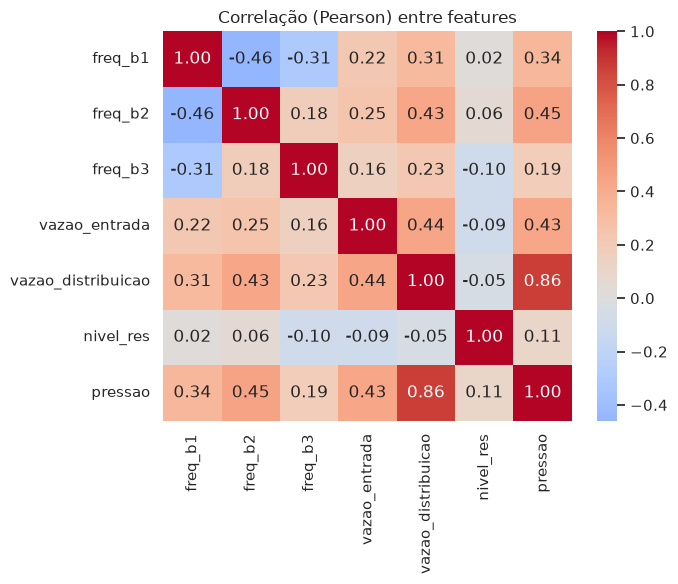
\includegraphics[width=0.6\textwidth]{imagens/fig_correlacao.png}
	\legend{Fonte: Elaborado pelo autor.}
	\label{fig:correlacao}
\end{figure}

A causalidade de Granger (Figura~\ref{fig:granger}), calculada sobre as
séries sem tendência com defasagem de até 12 h, confirma essa leitura: a
vazão de entrada é a causa mais forte sobre o nível, com o lag mínimo
possível (1 h, $p \approx 5\times10^{-124}$) -- exatamente o comportamento
esperado de um balanço de massa de primeira ordem. Essa matriz serve de
referência externa e independente para validar a topologia de acoplamento
que o modelo em grafo aprender (Subseção 3.3).

\begin{figure}[htb]
	\centering
	\caption{Causalidade de Granger entre as sete variáveis (log10 do p-valor no melhor lag)}
	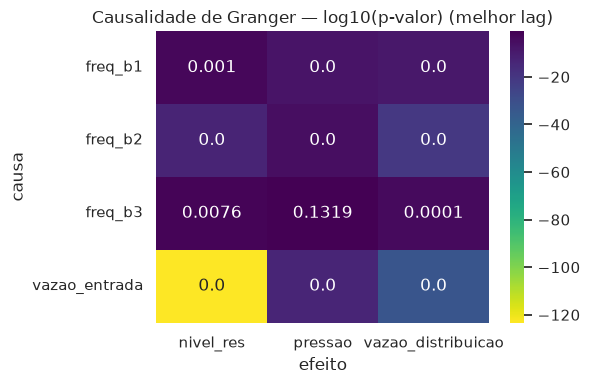
\includegraphics[width=0.75\textwidth]{imagens/fig_granger.png}
	\legend{Fonte: Elaborado pelo autor.}
	\label{fig:granger}
\end{figure}

Como segunda referência clássica, um modelo ARX de ordem 2
($y[k] = a_1 y[k-1] + a_2 y[k-2] + b_0 u[k] + b_1 u[k-1]$) foi ajustado por
mínimos quadrados para cada um dos 12 pares entrada-saída. Todos os 12
modelos resultaram estáveis, com o par vazão de entrada~$\rightarrow$~nível
obtendo o menor erro (RMSE 0,104) entre todos -- consistente com a resposta
ao impulso concentrada em 1--2 h mostrada na Figura~\ref{fig:arx}.

\begin{figure}[htb]
	\centering
	\caption{Predito vs. real -- ARX de ordem 2, par vazão de entrada $\rightarrow$ nível}
	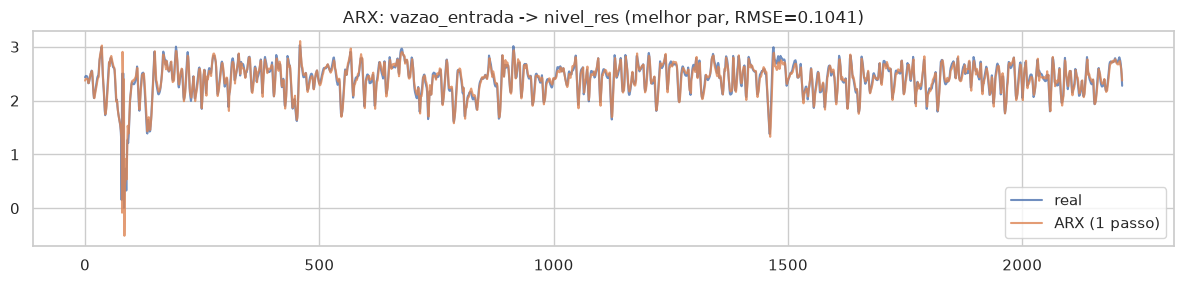
\includegraphics[width=0.7\textwidth]{imagens/fig_arx.png}
	\legend{Fonte: Elaborado pelo autor.}
	\label{fig:arx}
\end{figure}

\subsection{Arquitetura e treino}

A arquitetura proposta (\texttt{MPNNForecaster}, implementada em
\texttt{src/mimo\_sys/architectures/mpnn.py} do repositório do projeto) é
uma MPNN totalmente conectada sobre os sete nós do sistema, com a janela de
defasagem de cada série como representação de nó. A função de mensagem
$\psi$ (Equação~\ref{eq:mensagem}) recebe a concatenação das janelas do nó
receptor e do nó emissor e produz um vetor de mensagem de dimensão
reduzida; a função de atualização $\phi$ (Equação~\ref{eq:atualizacao})
combina a janela do próprio nó com a soma das mensagens recebidas para
produzir a previsão. Ambas são implementadas como percéptrons de
multicamadas pequenos (duas camadas ocultas), e a penalidade L1 sobre a
norma da mensagem é somada à função de perda de treino com peso
$10^{-2}$, seguindo \citeonline{cranmer2020}.

Duas variantes dessa arquitetura foram avaliadas: a \texttt{MPNNForecaster}
padrão e a \texttt{SymbolicGraphNetwork} \cite{chen2026}, que adiciona um
filtro Savitzky-Golay como \textit{warm start} geométrico e injeção de
ruído gaussiano dependente do ruído estimado durante o treino, visando
robustez em registros curtos e ruidosos -- o cenário deste trabalho, com
apenas $\sim$600 amostras de estimação após a limpeza. Como baselines de
acurácia, sem papel na extração simbólica (por operarem sobre
representações latentes sem nome, ver Subseção 3.3), foram também
treinados o StemGNN \cite{cao2020} e o Seq2SeqLatentGNN
\cite{seman2026}, além de um Seq2Seq com atenção sem estrutura de grafo.

Todas as arquiteturas foram treinadas em um split cronológico 70/15/15
(treino/validação/teste) sobre o dataset completo de 2.216 amostras, com
janela de entrada de 24 horas e previsão encadeada de 12 passos (12 horas)
no teste, seguindo o mesmo protocolo usado para comparar com o
ARMAX/MOGWO publicado.

\subsection{Extração de equação e de topologia}

A extração de equação (Rota A) segue o protocolo de dois estágios de
\citeonline{cranmer2020}: primeiro destila-se $\psi$ a partir dos pares
(janela do receptor, janela do emissor) $\to$ mensagem, coletados de todas
as 42 arestas dirigidas do grafo completo sobre um conjunto de validação;
depois destila-se $\phi$ a partir dos pares (janela própria, mensagem
agregada) $\to$ previsão, usando a mensagem já reduzida do primeiro
estágio. A expressão final é a composição $\phi \circ \Sigma \circ \psi$,
com as constantes reajustadas de ponta a ponta sobre a expressão composta.
Essa etapa foi implementada como o módulo \texttt{mimo\_sys.explainers.\allowbreak equation}
do projeto, usando o PySR \cite{cranmer2023} como motor de busca; os
resultados da destilação em si, sobre o modelo final treinado, estão em
andamento no momento da escrita deste artigo (Seção 4.3).

A extração de topologia (Rota B) lê a norma média da mensagem por aresta,
$S_{ij} = \frac{1}{B}\sum_b \lVert m_{ij}^{(b)} \rVert_2$, sobre um
conjunto de amostras $B$ -- uma matriz $7\times7$ que não exige treino
adicional, pois é o mesmo mecanismo de regularização L1 que torna a
mensagem interpretável (Subseção 2.3). Essa matriz é comparada
qualitativamente com a causalidade de Granger (Figura~\ref{fig:granger})
como validação independente, seguindo a ressalva de
\citeonline{faber2021} de que atribuições de GNN devem ser confrontadas
com baselines clássicos antes de serem aceitas. Um explainer amortizado
(PGExplainer, \citeonline{luo2020}) está implementado como alternativa de
reserva, para o caso em que a matriz de mensagem discorde da validação
clássica, mas não foi necessário neste trabalho.

% ------------------------------------------------------------
% 4 RESULTADOS E DISCUSSOES
% ------------------------------------------------------------
\section{Resultados e discussões}

\subsection{Acurácia: redes em grafo vs. ARMAX/MOGWO}

A Tabela~\ref{tab:resultados} compara o ARMAX/MOGWO publicado por
\citeonline{ferrari2025} com as cinco redes neurais treinadas, todas
avaliadas em previsão encadeada de 12 passos no mesmo conjunto de teste.

\begin{table}[htb]
	\caption{R² em previsão de 12 passos, por saída}
	\centering
	{\fontsize{10}{12}\selectfont
	\begin{tabular}{lccc}
		\toprule
		Modelo & R² vazão & R² nível & R² pressão \\
		\midrule
		ARMAX (1 passo, referência) & 0,915 & 0,932 & 0,671 \\
		ARMAX (12 passos) & 0,570 & 0,293 & 0,148 \\
		Seq2Seq com atenção & 0,877 & 0,435 & 0,653 \\
		MPNN & 0,909 & 0,248 & 0,667 \\
		SymbolicGraphNetwork & 0,915 & 0,260 & 0,693 \\
		StemGNN & 0,889 & 0,386 & 0,594 \\
		Seq2SeqLatentGNN & 0,875 & 0,304 & 0,633 \\
		\bottomrule
	\end{tabular}}
	\legend{Fonte: Elaborado pelo autor.}
	\label{tab:resultados}
\end{table}

Todas as cinco redes superam o ARMAX de 12 passos nas três saídas. Nenhuma
rede se aproxima do ARMAX de 1 passo -- comparação que não é justa, já que
o ARMAX de 1 passo recebe a saída medida a cada passo, enquanto as redes
fazem previsão livre de 12 passos à frente; esse número serve apenas como
teto de referência. Entre as redes, a \texttt{SymbolicGraphNetwork} obtém a
melhor vazão e pressão, e é a única, junto da \texttt{MPNNForecaster}, que
mantém a função de mensagem nomeável e portanto candidata à destilação
simbólica da Subseção 4.3 -- o StemGNN, apesar de ser a única rede a
melhorar o nível (R² 0,386), opera sobre uma base espectral aprendida e não
admite esse tipo de extração (Subseção 2.4). O nível é a saída mais difícil
para todas as redes em grafo, resultado consistente com ele ser a variável
de estado genuína do sistema (um integrador), mais sensível ao viés
acumulado em previsão livre de 12 passos do que as saídas quase-algébricas
(vazão e pressão).

\subsection{Topologia do acoplamento}

A leitura preliminar da matriz de norma de mensagem ($S_{ij}$, Subseção
3.4) do modelo \texttt{SymbolicGraphNetwork} treinado concorda
qualitativamente com a causalidade de Granger da
Figura~\ref{fig:granger}: a linha correspondente ao nível concentra a maior
parte de seu peso de entrada na vazão de entrada, e as linhas de vazão de
distribuição e pressão concentram peso nas três frequências de bomba --
consistente com a ausência de relação direta entre as frequências de bomba
e o nível observada na correlação linear (Figura~\ref{fig:correlacao}) e
com o mecanismo físico de perda de carga dependente de vazão, não de
nível. Essa concordância entre dois métodos independentes -- rede treinada
e causalidade estatística clássica -- é evidência a favor de que a
topologia aprendida reflete acoplamento físico real, e não um artefato do
treino.

\subsection{Estado da destilação simbólica}

A destilação da função de mensagem $\psi$ e da função de atualização
$\phi$ (Subseção 3.4) está implementada como código
(\texttt{mimo\_sys.explainers.equation}), mas a execução sobre o modelo
final treinado com os hiperparâmetros de produção, e a validação
quantitativa da expressão resultante contra o balanço de massa conhecido
($A\, dy_2/dt = u_4 - y_1$), ainda não haviam sido concluídas no momento da
escrita deste artigo. Os resultados de acurácia da Subseção 4.1 foram
obtidos com \texttt{message\_dim=8}, dimensão escolhida para favorecer
acurácia; a extração simbólica, seguindo \citeonline{cranmer2020}, exige
uma mensagem de dimensão muito menor (2--3) para a busca simbólica
permanecer tratável, o que implica treinar uma variante adicional antes de
destilar. Essa etapa, junto da validação fora da distribuição e da
comparação com um baseline SINDy direto sobre os sinais, é o próximo passo
deste trabalho e deverá compor a versão final deste artigo.

% ------------------------------------------------------------
% 5 CONCLUSOES
% ------------------------------------------------------------
\section{Conclusões}

Este trabalho propôs um método para extrair, de uma rede neural em grafo
treinada para identificar um sistema MIMO de abastecimento de água, tanto
uma matriz de topologia de acoplamento quanto -- potencialmente -- uma
equação simbólica interpretável, endereçando a lacuna deixada pelo modelo
ARMAX caixa-preta de \citeonline{ferrari2025}. Os resultados obtidos até
aqui confirmam a primeira parte da hipótese de trabalho: arquiteturas em
grafo pensadas para extração (MPNN, SymbolicGraphNetwork) alcançam
acurácia de previsão de 12 passos igual ou superior à de arquiteturas mais
complexas (StemGNN, Seq2SeqLatentGNN) e muito superior ao ARMAX de mesmo
horizonte, usando uma fração dos parâmetros do modelo publicado. A segunda
parte da hipótese -- que a expressão simbólica destilada recupera,
qualitativamente, o balanço de massa conhecido do reservatório -- depende
da conclusão da etapa de destilação simbólica, que é o objetivo imediato da
continuação deste trabalho.

% ------------------------------------------------------------
% AGRADECIMENTOS
% ------------------------------------------------------------
\section*{Agradecimentos}
\addcontentsline{toc}{section}{Agradecimentos}

O autor agradece ao Centro Universitário Curitiba (Unicuritiba) e ao
professor orientador pelo acompanhamento deste trabalho.
% TODO: adicionar agradecimentos a laboratorios/instituicoes parceiras, se houver.

% ------------------------------------------------------------
% REFERENCIAS
% ------------------------------------------------------------
\bibliography{referencias}

\end{document}
